\documentclass{article}
\usepackage[utf8]{inputenc}
\usepackage{amsmath}
\usepackage{scrextend}
\usepackage{setspace}
\usepackage{amsfonts}
\usepackage{amssymb}
\usepackage{graphicx}
\graphicspath{ {./} }

\title{Linear Algebra Done Right\\
\large{HW 3}}
\author{shaozewxy }
\date{June 2022}

\doublespacing
\begin{document}

\maketitle

\setcounter{secnumdepth}{0}
\section{3.1}
(Axler 3B.2)\\
$\forall v \in V, ST(v) \in range\ S \rightarrow ST(v) \in null\ T \rightarrow TST(v) = 0 \rightarrow STST(v) = S(0) = 0$\\
Therefore $(ST)^2 = 0$.
\section{3.2}
(Axler 3B.12)\\
Let $v_1, ..., v_n$ a basis of $null\ T$, then extend it to $v_1, ..., v_n, u_1, ..., u_m$ a basis of $V$.\\
Let $U = span(u_1, ..., u_m)$, then we claim $U \cap null\ T = \{0\}$ and $range\ T = \{Tu:u \in U\}$.\\
Suppose $v \neq 0 \in U \cap null\ T$, then this means $\exists a_1v_1 + ... + a_nv_n = v = b_1u_1 + ... + b_mu_m \rightarrow a_1v_1 + ... + a_nv_n - b_1u_1 - ... - b_mu_m = 0$, contradictory to $v_1, ..., v_n, u_1, ..., u_m$ a basis, therefore $U \cap null\ T = \{0\}$\\
Given $w \in range\ T, \exists v = a_1v_1 + ... + a_nv_n + b_1u_1 + ... + b_mu_m \in V$ such that $ Tv = w$, then we create $u = b_1u_1 + ... + b_mu_m \in U$ and $Tu = Tv = w$, therefore $range\ T \subseteq \{Tu: u \in U\}$ and therefore $range\ T = \{Tu: u \in U\}$.
\section{3.3}
(Axler 3B.20)\\
Suppose $T$ injective. NTS $\exists S \in \mathcal{L}(W, V)$ such that $ST = 1$.\\
Create $S':range\ T \rightarrow V$ by
\begin{equation*}
    S'(u) = v | Tv(u)
\end{equation*}
This is possible because $T$ injective, and therefore $\exists ! v \in V, Tv = u$.\\
Then it is obvious that we can extend $S'$ to linear map $S \in \mathcal{L}(V, W)$.\\
Then $\forall v \in V, ST(v) = S(T(v)) = v$, therefore $ST = 1$.\\
Suppose $\exists S \in \mathcal{L}(W, V)$ such that $ST = 1$, NTS $T$ injective.\\
$\forall u, v \in V$ such that $Tu = Tv$, then we have $S(T(v)) = S(T(u)) \rightarrow v = u$. Therefore $T$ injective.
\section{3.4}
(Axler 3B.21)\\
Suppose $T$ surjective. NTS $\exists S \in \mathcal{L}(W, V)$ such that $ST = 1$.\\
Create $S \in \mathcal{L}(W, V)$ with
\begin{equation*}
    S(w) = v | Tv = w
\end{equation*}
This is possible because $T$ surjective.\\
Then $\forall w \in W, TS(w) = T(S(w)) = T(v)$ with $Tv = w$, therefore $TS(w) = w$, therefore $TS = 1$.\\
Suppose $\exists S \in \mathcal{L}(W, V)$ such that $TS = 1$, NTS $T$ surjective.\\
$\forall w \in W, T(S(w)) = w$ therefore $T$ surjective.
\section{3.5}
(Axler 3B.29)\\
First NTS $null\ \phi, U = \{au:a \in \mathbf{F}\}$ are independent:\\
Suppose $\exists v \neq 0 \in null\ \phi \cap U$, then this $v = au, a \neq 0$ and therefore $\phi(au) = a \phi(u) = 0 \rightarrow \phi(u) = 0$, contradiction. Therefore $null\ \phi$ independent from $U$.\\
Then NTS $null\ \phi + U = V$:\\
Suppose $v_1, ..,, v_n$ a basis of $null\ \phi$. Because $\exists u \in V$ such that $\phi(u) \neq 0 \in \mathbf{F}$, this means $dim\ range\ \phi > 0$ and because $dim\ \mathbf{F} = 1$, we have that $0 < dim\ range\ \phi \leq 1 \rightarrow dim\ range\ \phi = 1$.\\
Therefore $dim\ V = dim\ null\ \phi + dim\ range\ \phi = n+1$. We can extend $v_1, ..., v_n$ to $v_1, ..., v_n, u$ to claim this is a basis of $V$:
First as proved before, $U = \{au: a \in \mathbf{F}\} = span(\{u\})$ is independent from $null\ \phi$, therefore $v_1, ..., v_n, u$ is linearly independent, because $dim \{v_1, ..., v_n, u\} = n+1 = dim\ V$ and $v_1, ..., v_n, u$ linearly independent, this means $v_1, ..., v_n, u$ a basis of $V$ and therefore $null\ \phi + U = V$.\\
Therefore $null\ \phi \oplus U = V$
\section{3.6}
(Axler 3C.3)\\
Given $T \in \mathcal{L}(V, W)$, we first create $v_1, ..., v_n$ a basis of $null\ T$, then we extend it to $u_1, ..., u_j, v_1, ..., v_n$ a basis of $V$.\\
Then we take $u_1, ..., u_j$ and create $Tu_1, ..., Tu_j$ a basis for $range\ T$, then extend it to $Tu_1, ..., Tu_j, w_1, ..., w_m$ a basis of $W$.\\
Then $\mathcal{M}(T)$ given these two basis will satisfy the requirements.
\section{3.7}
(Axler 3D.7)\\
1. If $v = 0$, then $\forall T \in \mathcal{L}(V, W), T(v) = 0$, i.e. $E = \mathcal{L}(V, W)$ and $E$ obviously a subspace of $\mathcal{L}(V, W)$.\\
If $v \neq 0$, then $\forall T, S \in E, \forall \lambda \in \mathbf{F}, T+S(v) = Tv + Sv = 0 + 0 = 0, \lambda T(v) = \lambda(Tv) = \lambda 0 = 0$, therefore $E$ closed under addition and scalar multiplication, and therefore a subspace.\\
2. Given $v \neq 0$, extend it to $v, v_1, ..., v_{n-1}$ a basis of $V$, and suppose $w_1, ..., w_m$ a basis for $W$, then we can see that $dim\ E = (n-1)m$.
\section{3.8}
(Axler 3D.16)\\
Given $v_1, ..., v_n$ a basis of $V$, define $S \in \mathcal{L}(V)$ as
\begin{equation*}
    S(v) = \begin{cases}
    v_1 & v = v_1 \\
    0 & \textrm{otherwise}
    \end{cases}
\end{equation*}
Then suppose $T(v_1) = \sum_{i=1}^{n} a_iv_i$, we have $ST(v_1) = S\left(\sum_{i=1}^{n} a_iv_i\right) = S(a_1v_1) = a_1v_1 = TS(v_1) = T(v_1) = \sum_{i=1}^{n} a_iv_i$, i.e.
\begin{equation*}
    a_1v_1 = \sum_{i=1}^{n}a_iv_i
\end{equation*}
From this we can get $a_2, ..., a_n = 0$, i.e. $T(v_1) = a_1v_1$, similarly we can say that $T$ is defined as
\begin{equation*}
    T(v_i) = a_iv_i
\end{equation*}
Now we NTS $a_1 = a_2 = ... = a_n$.\\
Create $S \in \mathcal{L}(V)$ as
\begin{equation*}
    S(v) = \begin{cases}
    v_2 & v = v_1 \\
    0 & \textrm{otherwise}
    \end{cases}
\end{equation*}
Then we have that $TS(v_1) = T(v_2) = a_2v_2 = ST(v_1) = S(a_1v_1) = a_1v_2 \rightarrow a_1 = a_2$. Similarly we have $a_1 = a_2 = ... = a_n$.\\
Then $T$ can defined as
\begin{equation*}
    T(v_i) = av_i
\end{equation*}
i.e. $T$ is a scalar multiple of identity.
\section{3.9}
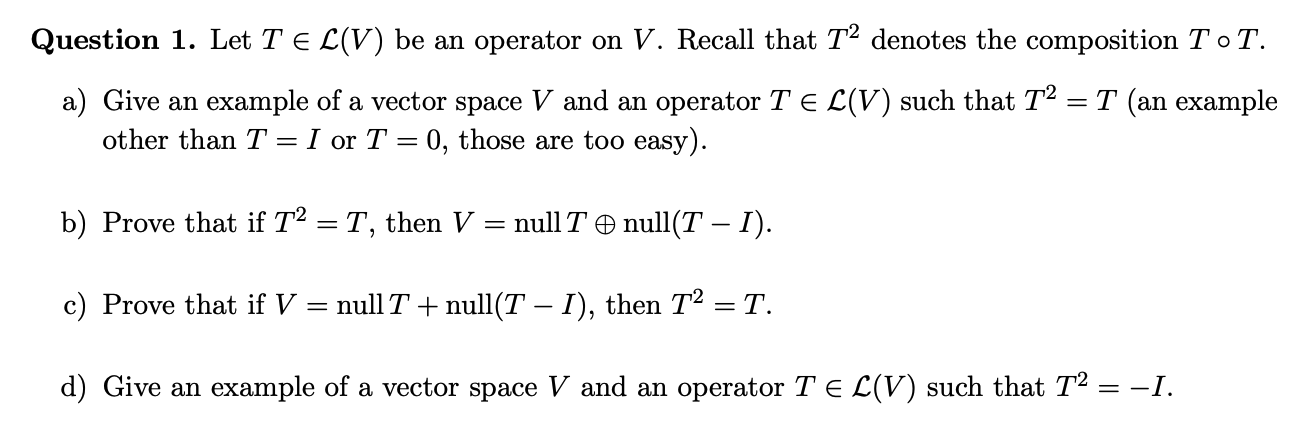
\includegraphics[scale=0.5]{q3_1.png}
a. Let $V = \mathbb{R}^2$ and $v_1 = (1, 0)^t, v_2 = (0, 1)^t$ be a basis of $V$. Then define $T \in \mathcal{L}(V)$ as
\begin{equation*}
    Tv_1 = 0, Tv_2 = v_2
\end{equation*}
Then $\forall v = a_1v_1 + a_2v_2 \in V, Tv = a_2v_2, T^2v = T(Tv) = a_2v_2 = Tv$.\\
b. Given $T^2 = T$, first NTS $null\ T, null\ (T-I)$ independent:\\
Suppose $\exists v \in nul\ T \cap nul\ (T-I)$, then $Tv = 0, (T-I)v = 0 \rightarrow v = Iv = Tv = 0$. Therefore $nul\ T, nul\ (T-I)$ independent.\\
Then NTS $nul\ T + nul\ (T-I) = V$:\\
We show that there is a bijection between $nul\ (T-I)$ and $range\ T$:\\
$\forall Tv \in range\ T$, because $T(Tv) = Tv \rightarrow Tv \in nul\ (T-I)$, i.e. $\exists Tv \in nul\ (T-I)$ such that $T(Tv) = Tv$, the mapping surjective.\\
$\forall v_1 \neq v_2 \in nul\ (T-I), Tv_1 = v_1 \neq v_2 = Tv_2$, i.e. the mapping injective.\\
Therefore $\exists$ a bijection between $range\ T, nul\ (T-I)$, i.e. $dim\ nul\ (T-I) = dim\ range\ T$.\\
Therefore $V = nul\ T \oplus nul\ (T-I)$.\\
c. This is obvious. Given $v \in V$, if $v \in nul\ T$, then obviously $Tv = 0 = T(Tv)$. So assume $v \in nul\ (T-I)$, then we have $Tv = v \rightarrow T(Tv) = Tv$, i.e. $\forall v \in V, T^2 = T$.\\
d. Let $V = \mathbb{R}^2$, with $v_1 = (1, 0)^t, v_2 = (0, 1)^t$ be the basis. Then we define $T \in \mathcal{L}(V)$ as the mapping given by
\begin{equation*}
    \mathcal{M}(T) = \begin{pmatrix}
    0 & 1\\
    -1 & 0
    \end{pmatrix}
\end{equation*}
Given $v = a_1v_1 + a_2v_2 = (a_1, a_2)^t \in V$,
\begin{equation*}
    Tv = \begin{pmatrix}
    0 & 1\\
    -1 & 0
    \end{pmatrix}
    \begin{pmatrix}
    a_1\\
    a_2
    \end{pmatrix} = 
    \begin{pmatrix}
    a_2\\
    -a_1
    \end{pmatrix}
\end{equation*}
Therefore $T^2(v) = (-a_1, -a_2)^t = -v$
\section{3.10}
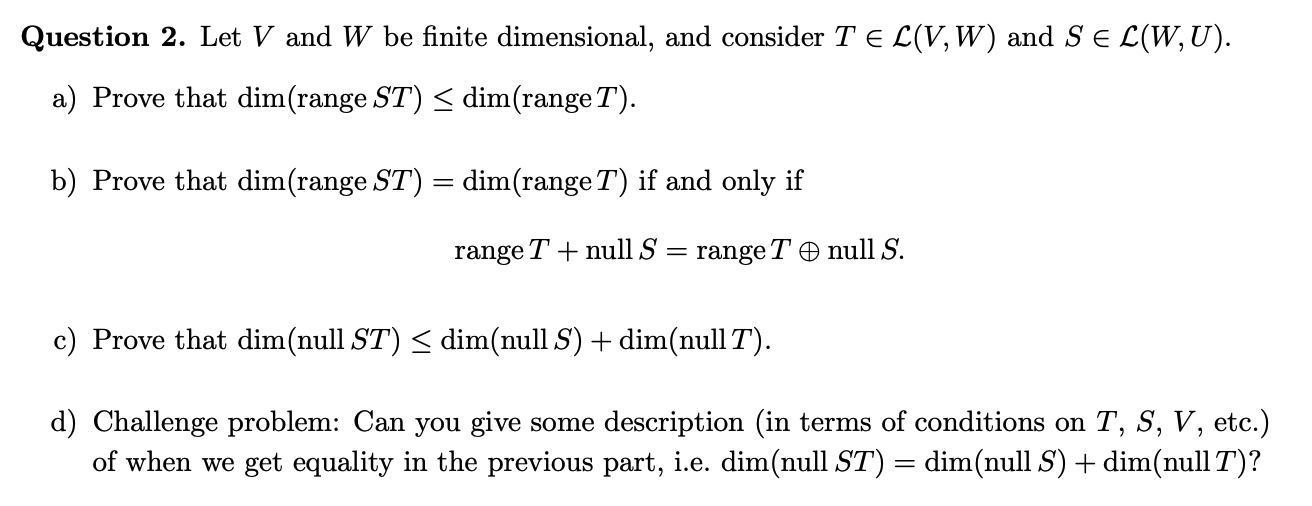
\includegraphics[scale=0.5]{q3_2.png}
a. $ST \in \mathcal{L}(V, U)$, therefore $dim\ range\ ST = dim\ V - dim\ nul\ ST, dim\ range\ T = dim\ V - dim\ nul\ T$.\\
$\forall v \in nul\ T, Tv = 0 \rightarrow ST(v) = S(Tv) = S(0) = 0 \rightarrow v \in nul\ ST$, i.e. $nul\ T \subseteq nul\ ST \rightarrow dim\ nul\ T \leq dim\ nul\ ST$.\\
Therefore $dim\ range\ ST \leq dim\ range\ T$.\\
b. If $range\ T, nul\ S$ independent, NTS $dim\ range\ ST = dim\ range\ T$:\\
From a, we know only NTS $nul\ T = nul\ ST$, i.e. $nul\ ST \subseteq nul\ T$:\\
$\forall v \in nul\ ST, ST(v) = S(Tv) = 0 \rightarrow Tv \in nul\ S$, but since $range\ T, nul\ S$ independent, therefore $Tv = 0 \rightarrow v \in nul\ T$. Therefore $nul\ ST \subseteq nul\ T$, and thus $nul\ ST = nul\ T$ and $dim\ range\ ST = dim\ range\ T$.\\
If $dim\ range\ ST = dim\ range\ T$, then NTS $range\ T, nul\ S$ independent:\\
Again $nul\ ST = nul\ T$. Suppose $\exists w \in range\ T \cap nul\ S$, then this means $\exists v \in V$ such that $Tv = w$, i.e. $ST(v) = S(Tv) = S(w) = 0$, i.e. $v \in nul\ ST \rightarrow v \in nul\ T \rightarrow w = Tv = 0$. Therefore $range\ T, nul\ S$ independent.\\
c. We define $T' \in \mathcal{L}(T^{-1}(nul\ S), nul\ S)$ as
\begin{equation*}
    T'v = Tv
\end{equation*}
Then we have $dim\ T^{-1}(nul\ S) = dim\ nul\ T' + dim\ range\ T'$.\\
First show $nul\ T' = nul\ T$:\\
$\forall v \in nul\ T, ST(v) = S(0) = 0 \rightarrow v \in T^{-1}(nul\ S)$ and since $T'(v) = T(v) = 0$, we have $v \in nul\ T'$, i.e. $nul\ T \subseteq nul\ T'$.\\
Since obviously $nul\ T' \subseteq nul\ T$, we have $nul\ T = nul\ T'$.\\
Then since obviously $T^{-1}(nul\ S) = nul\ ST$ and $range\ T' \subseteq nul\ S$, we have:
\begin{equation*}
    dim\ nul\ ST = dim\ T^{-1}(nul\ S) = dim\ nul\ T' + dim\ range\ T'
\end{equation*}
\begin{equation*}
    = dim\ nul\ T + dim\ range\ T' \leq dim\ nul\ T + dim\ nul\ S
\end{equation*}
d. From c., we can know that this achieves equality when $range\ T' = nul\ S$.
\end{document}